% Paper 2 of the SurvX project. Draft for Biometrical Journal.
% Generic article layout; move to the Wiley NJD template (WileyNJD-v2.cls) at submission.
\documentclass[11pt]{article}
\usepackage[a4paper,margin=2.5cm]{geometry}
\usepackage[T1]{fontenc}
\usepackage{lmodern}
\usepackage{amsmath,amssymb,amsthm,bm}
\usepackage{graphicx,booktabs,multirow,array}
\usepackage[authoryear,round]{natbib}
\usepackage{xcolor}
\usepackage{tikz}
\usetikzlibrary{positioning,arrows.meta,calc}
\usepackage[hidelinks]{hyperref}
\usepackage{lineno}
\linenumbers
\usepackage{setspace}
\onehalfspacing

\newtheorem{proposition}{Proposition}
\newtheorem{remark}{Remark}
\newcommand{\tbd}[1]{\textcolor{red}{[TBD: #1]}}
\newcommand{\E}{\mathrm{E}}
\newcommand{\I}{\mathrm{I}}
\newcommand{\T}{\top}
\newcommand{\Ghat}{\widehat G}

\title{Direct parametric regression for cumulative incidence functions:\\
a weighted estimator with a corrected variance, and a coherent model for several causes}
\author{Habib Ezzatabadipour\thanks{\tbd{affiliation}. E-mail: habibezati@outlook.com}}
\date{}

\begin{document}
\maketitle

\begin{abstract}
\noindent
Parametric models for the cumulative incidence function (CIF) give smooth absolute risks and, with
baselines that level off, an estimate of the long-run probability of each type of event. Two
problems limit their use. First, the full likelihood of Jeong and Fine models every cause, so a
wrong model for a competing cause biases the cause of interest. Second, separately specified
models for the CIFs need not add up to at most one; with several causes the predicted long-run
risks of many subjects add up to more than one. We address both. For a single cause we study a
weighted estimator in which subjects who fail from a competing cause enter through the
Kaplan--Meier estimate of the censoring distribution, as in Fine and Gray, and we derive the
exact sandwich variance that accounts for the estimated censoring distribution: a closed form of
the infinitesimal jackknife. For $K \ge 3$ causes we propose a constrained model that keeps a
direct regression model for the cause of interest and shares the remaining long-run risk among the
competing causes by a multinomial logit, so that the CIFs add up to one at infinity and never
exceed one, for every covariate value; with two causes it reduces to the model of Shi, Cheng and
Jeong. In simulations the weighted estimator was unbiased with 93--97\% coverage when the joint
estimator, with the competing cause misspecified, covered as little as 74\%; the correction of
the variance changed the standard errors by at most 1.2\%. The constrained model gave coherent
predictions in every replication, whereas the unconstrained joint model gave long-run risks
adding up to more than one for 28--97\% of the subjects, and its long-run risks were unbiased
when its assumptions held. Data on time to live birth and on cause of death in the free light
chain cohort illustrate the methods, including a check of when long-run risks are identified.
All methods are implemented in the R package \texttt{SurvX}.

\medskip\noindent
\textbf{Keywords:} competing risks; cumulative incidence function; inverse probability of censoring
weighting; long-term incidence; sandwich variance.
\end{abstract}

% =====================================================================================
\section{Introduction}\label{sec:intro}
% =====================================================================================
With competing risks the cumulative incidence function (CIF), $F_k(t \mid z) = P(T \le t, \varepsilon = k \mid Z = z)$,
gives the probability of an event of type $k$ by time $t$ and is the quantity most often wanted
for prognosis \citep{putter2007,andersen2012}. The proportional subdistribution hazards model of
\citet{fine1999} is the standard regression model for it. Being semi-parametric, it leaves the
baseline CIF unspecified and does not by itself give a long-run risk $F_k(\infty \mid z)$, the
probability of ever experiencing the event, which is often of direct interest: the proportion of
women who ever have a live birth, the lifetime risk of death from a given cause.

Parametric models for the CIF fill this gap. \citet{jeong2006,jeong2007} proposed an improper
Gompertz baseline whose CIF levels off below one, combined with the generalized odds-rate
transformation of \citet{dabrowska1988}, which contains proportional subdistribution hazards and
proportional odds as special cases. \citet{cheng2009} proposed a modified three-parameter logistic
baseline, mixture forms $p\,G(t)$ with a proper distribution function $G$ go back to
\citet{larson1985}, and \citet{lambert2017} and \citet{mozumder2018} used restricted cubic splines
\citep{royston2002}. Estimation is either by the full likelihood of all causes jointly
\citep{jeong2007,mozumder2018} or by a weighted likelihood for one cause alone, in which subjects
who fail from a competing cause enter through the Kaplan--Meier estimate of the censoring
distribution as in \citet{fine1999}, \citet{geskus2011} and \citet{lambert2017}.

Two problems arise in practice. The first is robustness: the full likelihood needs a correct model
for every cause, so a poor model for a cause of no interest can bias the cause that matters. The
weighted estimator avoids this, but its usual sandwich variance treats the estimated censoring
distribution as known; the correction derived by \citet{fine1999} for the subdistribution hazards
model has, to our knowledge, not been worked out for parametric weighted estimators, and its size
in practice is not known. The second problem is coherence. Nothing forces separately specified
CIFs to add up to at most one. This is well documented for multiple Fine--Gray models
\citep{austin2021,bonneville2024}; with parametric models that level off it is acute, because
long-run risks are extrapolations and their sum over causes can be far above one.
\citet{shi2013} solved the coherence problem for two causes by modelling the cause of interest
directly and writing the competing CIF as $\{1 - F_1(\infty \mid z)\}\,G(t)$. No such model exists
for three or more causes, where the leftover probability must also be divided between the
competing causes.

This paper makes four contributions. (i) We describe the weighted estimator as an expected complete
data log-likelihood and give an evaluation that is linear in the sample size for proportional
subdistribution hazards. (ii) We derive the variance that accounts for the estimated censoring
distribution in closed form, as the exact infinitesimal jackknife of the estimator with the
Kaplan--Meier estimate recomputed; its continuous version has the form of the correction of
\citet{fine1999}. (iii) We propose a constrained model for $K \ge 3$ causes that combines a direct
model for the cause of interest with multinomial-logit shares of the remaining long-run risk, in
the spirit of \citet{larson1985}; its CIFs add up to one at infinity for every covariate value and
it reduces to \citet{shi2013} for $K = 2$. (iv) We evaluate all of this in a simulation study and
two applications, and we give a simple check of when long-run risks are identified by the data.
All methods are available in the R package \texttt{SurvX} \citep{ezzatabadipour2026}.

Section~\ref{sec:models} reviews the direct models. Section~\ref{sec:weighted} presents the
weighted estimator and its variance and Section~\ref{sec:constrained} the constrained model.
Section~\ref{sec:sim} reports the simulations and Section~\ref{sec:apps} the applications;
Section~\ref{sec:disc} discusses limitations. Proofs and further results are in the appendices.

% =====================================================================================
\section{Direct parametric models for the CIF}\label{sec:models}
% =====================================================================================
\subsection{Data and notation}
Let $T$ be the event time, $\varepsilon \in \{1, \dots, K\}$ the type of event, $C$ the censoring
time and $Z$ a $p$-vector of covariates. We observe $n$ independent copies of
$(X, \delta, Z)$ with $X = T \wedge C$ and $\delta = \varepsilon\,\I(T \le C)$, so that
$\delta = 0$ denotes censoring. Censoring is independent of $(T, \varepsilon)$ given $Z$, and
for the weighted estimator also independent of $Z$, with survival function $G(t) = P(C > t)$.
The CIF of type $k$ is $F_k(t \mid z)$, its density $f_k(t \mid z)$, and
$S(t \mid z) = 1 - \sum_k F_k(t \mid z)$ is the probability of no event by $t$. We call
$p_k(z) = F_k(\infty \mid z)$ the long-run risk of type $k$.

\subsection{Baselines and links}
Following \citet{jeong2007}, a direct model for the CIF of type $k$ is
\begin{equation}\label{eq:gor}
F_k(t \mid z) = 1 - \{1 + \alpha_k e^{\beta_k^\T z} u_k(t)\}^{-1/\alpha_k}, \qquad
F_k(t \mid z) = 1 - \exp\{-e^{\beta_k^\T z} u_k(t)\} \ (\alpha_k = 0),
\end{equation}
where $u_k$ is a non-decreasing baseline function with $u_k(0) = 0$. Equivalently,
$g_{\alpha}\{F_k(t \mid z)\} = \log u_k(t) + \beta_k^\T z$ with the generalized odds-rate link
$g_\alpha(x) = \log[\{(1-x)^{-\alpha} - 1\}/\alpha]$ of \citet{dabrowska1988}. The link $\alpha = 0$
gives proportional subdistribution hazards (PH), in which $e^{\beta}$ is a subdistribution hazard
ratio as in \citet{fine1999}; $\alpha = 1$ gives proportional odds (PO) of the CIF; with $\alpha$
estimated (GOR) the data choose the scale. We allow $\alpha < 0$ as long as
$1 + \alpha e^{\beta^\T z} u(t) > 0$ on the support.

The baselines considered here have a plateau, $u_k(\infty) < \infty$, so that $p_k(z) < 1$:
\begin{itemize}
\item the improper Gompertz $u(t) = \tau(e^{\rho t} - 1)/\rho$ with $\rho < 0$ \citep{jeong2006};
\item mixture baselines whose CIF at $z = 0$ is $F_0(t) = p\,G(t)$ with $G$ a Weibull,
log-logistic or log-normal distribution function \citep{larson1985,cheng2009}, so that
$u(t) = \exp[g_\alpha\{p\,G(t)\}]$;
\item the modified three-parameter logistic baseline CIF
$F_0(t) = p\,\{e^{b(t-c)} - e^{-bc}\}/\{1 + e^{b(t-c)}\}$ of \citet{cheng2009}.
\end{itemize}
For baselines specified as a CIF, $F_0$ is the CIF at $z = 0$, so continuous covariates are centred.

\subsection{Joint likelihood and the coherence problem}
With a model of the form \eqref{eq:gor} for every type, the joint estimator maximises
\begin{equation}\label{eq:joint}
\ell(\theta) = \sum_{i=1}^n \Big[\sum_{k=1}^K \I(\delta_i = k)\log f_k(X_i \mid Z_i)
  + \I(\delta_i = 0) \log S(X_i \mid Z_i)\Big]
\end{equation}
\citep{jeong2007}. Two features matter here. A misspecified model for one type enters $S$ and
biases the others. And nothing in \eqref{eq:joint} keeps $\sum_k F_k(t \mid z) \le 1$ except at the
censoring times of the sample, where $\log S$ must be finite; for other covariate values, or for
$t$ beyond follow-up, and in particular at $t = \infty$, the sum can exceed one. \texttt{SurvX}
reports this, and can restrict the optimisation to parameters with
$\sum_k F_k(t \mid Z_i) < 1$ for all $t$ up to the largest observed time and every subject in the
sample, but this does not make the long-run risks coherent. Section~\ref{sec:constrained} does.

% =====================================================================================
\section{The weighted estimator for one cause}\label{sec:weighted}
% =====================================================================================
\subsection{An expected complete-data likelihood}
Take type 1 as the type of interest and write $F = F_1$, $S_1 = 1 - F_1$ and $\theta$ for its
parameters. If every censoring time were known, the subdistribution time $T^* = T$ if
$\varepsilon = 1$ and $T^* = \infty$ otherwise \citep{fine1999} would be observed up to censoring at
$C \wedge \tau$, where $\tau$ is the largest observed time, and its log-likelihood would be
\begin{equation}\label{eq:complete}
\sum_i \Big[ \I(\delta_i = 1)\log f(X_i \mid Z_i) + \I(\delta_i \ne 1) \log S_1(C_i \wedge \tau \mid Z_i) \Big].
\end{equation}
For subjects censored, $C_i = X_i$. For subjects who failed from a competing cause ($\delta_i \ge 2$),
$C_i$ is unknown but larger than $X_i$. We replace their term by its conditional expectation given
$C_i \ge X_i$ under the Kaplan--Meier estimate $\Ghat$ of $G$. Let $c_1 < \dots < c_m$ be the
distinct censoring times, $c_{m+1} = \tau$, $\Ghat_r = \Ghat(c_r)$, $\Ghat_0 = 1$, and give
$c_r$ the mass $\mu_r = \Ghat_{r-1} - \Ghat_r$ ($r \le m$) and $c_{m+1}$ the remaining mass
$\mu_{m+1} = \Ghat_m$. For a competing failure let $f_i = \min\{r : c_r \ge X_i\}$ (failures
precede censorings at ties). The weighted log-likelihood is
\begin{equation}\label{eq:wll}
\begin{aligned}
\ell_w(\theta) = \sum_i \Big[ &\I(\delta_i = 1) \log f(X_i \mid Z_i) + \I(\delta_i = 0) \log S_1(X_i \mid Z_i)\\
 &+ \I(\delta_i \ge 2) \sum_{r \ge f_i} w_{ir} \log S_1(c_r \mid Z_i) \Big],
 \qquad w_{ir} = \frac{\mu_r}{\Ghat_{f_i - 1}}.
\end{aligned}
\end{equation}
The weights of a subject add up to one. Since the expectation of the complete-data score given
the observed data and $C_i \ge X_i$ is still zero at the true $\theta$ when $G$ is known, the
score $U(\theta; G) = \partial \ell_w / \partial\theta$ is an unbiased estimating function; with
$\Ghat$ in place of $G$ the estimator $\hat\theta$, the root of $U(\theta; \Ghat) = 0$, is consistent
under the usual positivity condition $G(\tau) > 0$. Equation \eqref{eq:wll} is the expanded-data
form used by \citet{geskus2011} and \citet{lambert2017}, written for the support of $\Ghat$. No model
for the competing causes is needed, and $\ell_w$ is a pseudo-likelihood: differences of $\ell_w$
between baselines or links can rank fits but have no likelihood-ratio interpretation.

\subsection{Fast evaluation}\label{sec:fast}
Evaluated directly, the inner sum in \eqref{eq:wll} costs $O(nm)$ operations for each value of
$\theta$. With the PH link, $\log S_1(c \mid z) = -e^{\beta^\T z} u(c)$, so
\[
\sum_{r \ge f_i} w_{ir} \log S_1(c_r \mid Z_i) = -\frac{e^{\beta^\T Z_i}}{\Ghat_{f_i - 1}} \, V_{f_i},
\qquad V_r = \sum_{r' \ge r} \mu_{r'} u(c_{r'}),
\]
and the suffix sums $V_r$, together with their first and second derivatives with respect to the
baseline parameters, are computed once per iteration in $O(m)$ operations. The log-likelihood,
score and observed information then cost $O(n + m)$. For the spline baseline the same holds with
suffix sums of $\mu_r e^{s_r}(1, s_r', s_r s_r'^\T)$, where $s_r$ is the spline basis at $\log c_r$.
For $\alpha \ne 0$ the sum does not separate; $u(c_r)$ and its derivatives are still computed
once per iteration, so each (subject, support point) pair needs only closed-form derivatives of
the link. Both paths agree with direct evaluation to $10^{-9}$.

\subsection{Variance with an estimated censoring distribution}\label{sec:psi}
The usual robust variance \citep{white1982} is $\hat A^{-1} \hat B \hat A^{-1}$ with
$\hat A = -\partial U/\partial \theta^\T$ and $\hat B = \sum_i U_i U_i^\T$, where $U_i$ is the
contribution of subject $i$ to $U(\hat\theta; \Ghat)$. It treats $\Ghat$ as known. We account for
$\Ghat$ through the infinitesimal jackknife \citep{efron1982}. Give subject $i$ a case weight $v_i$
in \eqref{eq:wll} and in the Kaplan--Meier estimate. Let $R_r = \sum_j v_j Y_j(c_r)$ with
$Y_j(c_r) = \I\{X_j > c_r \text{ or } (X_j = c_r, \delta_j = 0)\}$ be the number at risk of
censoring at $c_r$, $D_r = \sum_j v_j \I(X_j = c_r, \delta_j = 0)$ the number censored there, and
$\lambda_r = \log\{(R_r - D_r)/R_r\}$, so that $\log \Ghat_r = \sum_{q \le r} \lambda_q$. Write
$b_{ir} = \partial \log S_1(c_r \mid Z_i)/\partial\theta$ for $r \le m + 1$.

\begin{proposition}\label{prop:psi}
At $v = (1, \dots, 1)$, the derivative of $\hat\theta(v)$ with respect to $v_i$ is
$D_i = \hat A^{-1}(U_i + \psi_i)$, with
\begin{equation}\label{eq:psi}
\psi_i = \sum_{r=1}^{m} Q_r \frac{\partial \lambda_r}{\partial v_i}, \qquad
\frac{\partial \lambda_r}{\partial v_i} = \frac{Y_i(c_r)\, D_r}{R_r (R_r - D_r)} - \frac{\I(X_i = c_r, \delta_i = 0)}{R_r - D_r},
\end{equation}
\begin{equation}\label{eq:Q}
Q_r = \sum_{j : \delta_j \ge 2,\ f_j \le r} \ \sum_{r' = r}^{m} \frac{\Ghat_{r'}}{\Ghat_{f_j - 1}} \big(b_{j, r'+1} - b_{j r'}\big).
\end{equation}
The infinitesimal jackknife variance is
$\hat V = \sum_i D_i D_i^\T = \hat A^{-1} \big\{\sum_i (U_i + \psi_i)(U_i + \psi_i)^\T\big\} \hat A^{-1}$.
\end{proposition}

The proof (Appendix~\ref{app:psi}) uses summation by parts to write the contribution of a
competing failure as $b_{j f_j} + \sum_{r' \ge f_j} (\Ghat_{r'}/\Ghat_{f_j-1})(b_{j,r'+1} - b_{jr'})$,
which depends on $\Ghat$ only through $\lambda_{f_j}, \dots, \lambda_{m}$, and then the implicit
function theorem. Three remarks are in order.

\begin{remark}
$\psi_i$ is the exact derivative, not an approximation, and it agrees with numerical
differentiation of $\hat\theta(v)$ with the Kaplan--Meier estimate recomputed (Section~\ref{sec:valid}).
As $n \to \infty$, $\sum_r Q_r\,\partial\lambda_r/\partial v_i$ becomes $-\int q(s)\,
\pi(s)^{-1}\,dM_i^C(s)$ with $M_i^C$ the censoring martingale, $\pi(s) = P(X \ge s)$ and $q$
the limit of $n^{-1} Q$ per unit of censoring hazard: the form of the correction term in
\citet[Section~3.2]{fine1999}. We do not give a formal proof of the asymptotic normality of
$\hat\theta$; under the regularity conditions of \citet{fine1999} it follows from the functional
delta method for the Kaplan--Meier estimator, since $U$ is a smooth functional of $\Ghat$.
\end{remark}

\begin{remark}
Asymptotically, $\psi_i$ is minus the projection of the score onto the space spanned by the
censoring martingales \citep{tsiatis2006}, so the variance with the correction is no larger than the
variance that treats $G$ as known, as for inverse probability weighted estimators with an estimated
nuisance model \citep{robins1994}. In finite samples the estimated correction can go either way; in
the simulations it reduced the standard errors slightly (Section~\ref{sec:simA}), in the fertility
data it increased them by up to 0.5\%.
\end{remark}

\begin{remark}
$U_i$ depends on $\Ghat$ only for competing failures, so only their scores enter $Q_r$.
$\psi_i$ is computed once, after convergence.
\end{remark}

% =====================================================================================
\section{A coherent model for $K \ge 3$ causes}\label{sec:constrained}
% =====================================================================================
\subsection{The model}
Suppose every subject eventually experiences one of the $K$ events, as with death from one of
several causes. Keep a direct model \eqref{eq:gor} with a plateau for type 1, with long-run risk
$p_1(z) = F_1(\infty \mid z) < 1$, and let
\begin{equation}\label{eq:ck}
F_k(t \mid z) = \{1 - p_1(z)\}\,\pi_k(z)\,G_k(t), \qquad
\pi_k(z) = \frac{\exp(\gamma_k + \delta_k^\T z)}{\sum_{j=2}^K \exp(\gamma_j + \delta_j^\T z)},
\qquad k = 2, \dots, K,
\end{equation}
with $\gamma_2 = 0$, $\delta_2 = 0$ (the first competing type is the reference) and $G_k$ proper
distribution functions (Weibull, log-logistic or log-normal) with parameters $\phi_k$.
Figure~\ref{fig:concept} shows the structure. A subject eventually has an event of type 1 with
probability $p_1(z)$; otherwise, with probability $\pi_k(z)$, an event of type $k$ at a time
distributed as $G_k$. For $K = 2$, $\pi_2 \equiv 1$ and \eqref{eq:ck} is the model of
\citet{shi2013}.

\begin{figure}[t]
\centering
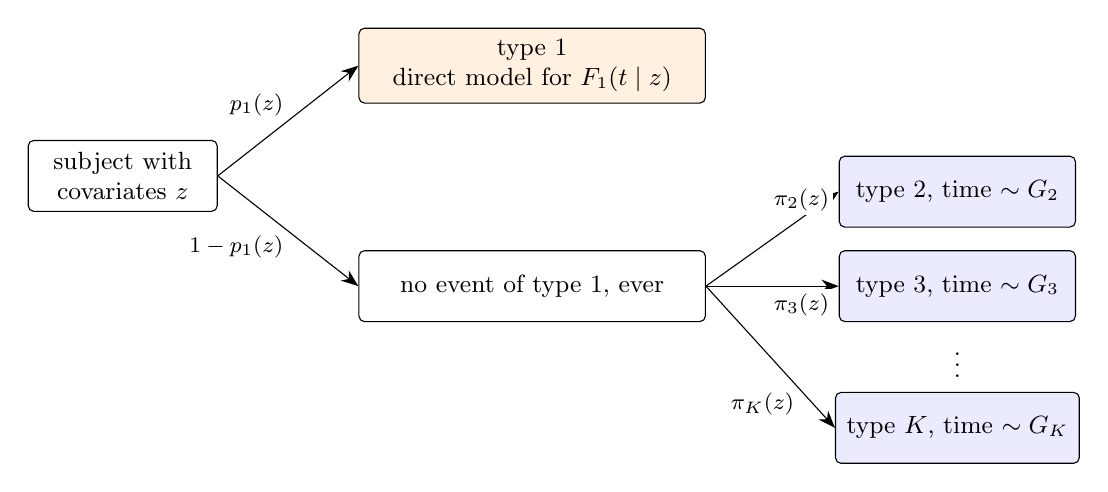
\begin{tikzpicture}[
  box/.style={draw, rounded corners=2pt, align=center, font=\small, inner sep=4pt, minimum height=9mm},
  lab/.style={font=\footnotesize, fill=white, inner sep=1.5pt},
  >={Stealth[length=2.2mm]}]
\node[box, minimum width=24mm] (s) at (0, 0) {subject with\\ covariates $z$};
\node[box, fill=orange!12, minimum width=44mm] (c1) at (5.2, 1.4) {type 1\\ direct model for $F_1(t \mid z)$};
\node[box, minimum width=44mm] (r) at (5.2, -1.4) {no event of type 1, ever};
\node[box, fill=blue!8, minimum width=30mm] (c2) at (10.6, -0.2) {type 2, time $\sim G_2$};
\node[box, fill=blue!8, minimum width=30mm] (c3) at (10.6, -1.4) {type 3, time $\sim G_3$};
\node[font=\small] (cd) at (10.6, -2.3) {$\vdots$};
\node[box, fill=blue!8, minimum width=30mm] (cK) at (10.6, -3.2) {type $K$, time $\sim G_K$};
\draw[->] (s.east) -- (c1.west) node[lab, pos=0.5, above left] {$p_1(z)$};
\draw[->] (s.east) -- (r.west) node[lab, pos=0.5, below left] {$1 - p_1(z)$};
\draw[->] (r.east) -- (c2.west) node[lab, pos=0.72, above=1pt] {$\pi_2(z)$};
\draw[->] (r.east) -- (c3.west) node[lab, pos=0.72, below=1pt] {$\pi_3(z)$};
\draw[->] (r.east) -- (cK.west) node[lab, pos=0.72, below left=0pt] {$\pi_K(z)$};
\end{tikzpicture}
\caption{The constrained model for $K$ types of event. Type 1 keeps a direct regression model with
long-run risk $p_1(z)$; the remaining probability is shared among the other types by a multinomial
logit $\pi_k(z)$ (type 2 the reference), each type with its own time distribution $G_k$. Hence
$\sum_k F_k(\infty \mid z) = p_1(z) + \{1 - p_1(z)\}\sum_{k \ge 2}\pi_k(z) = 1$ for every $z$.}
\label{fig:concept}
\end{figure}

\begin{proposition}\label{prop:coherent}
Under \eqref{eq:gor} with $u_1(\infty) < \infty$ and \eqref{eq:ck}, for every $z$:
(a) $\sum_{k=1}^K F_k(\infty \mid z) = 1$;
(b) $S(t \mid z) = \{p_1(z) - F_1(t \mid z)\} + \{1 - p_1(z)\}\sum_{k \ge 2} \pi_k(z)\{1 - G_k(t)\}$,
which is non-negative and non-increasing in $t$, so $\sum_k F_k(t \mid z) \le 1$ for all $t$;
(c) the model is that of a proper competing risks distribution in which every subject has an
event, with cause-specific hazards $h_k(t \mid z) = f_k(t \mid z)/S(t \mid z)$;
(d) for $K = 2$ it coincides with the model of \citet{shi2013}.
\end{proposition}
The proof is immediate from \eqref{eq:ck} and $\sum_{k \ge 2} \pi_k = 1$.

\subsection{Interpretation}
The coefficients $\beta_1$ keep the interpretation of the chosen link for type 1 (a subdistribution
hazard ratio for PH). For $k \ge 3$, $e^{\delta_k}$ is an odds ratio of having an event of type $k$
rather than type 2 among subjects who will not have an event of type 1. The effect of $z$ on the
long-run risk of a competing type combines both parts:
\[
\frac{\partial \log p_k(z)}{\partial z} = -\frac{\partial p_1(z)/\partial z}{1 - p_1(z)}
 + \delta_k - \sum_{j \ge 2} \pi_j(z)\, \delta_j, \qquad k \ge 2,
\]
so absolute risks from \texttt{predict()} are the natural summary. The time distributions $G_k$
do not depend on $z$; covariates act on the competing types through how much of the remaining
probability each receives, not through when.

\subsection{Estimation}
With $\xi = (\theta_1, \phi_2, \dots, \phi_K, \gamma_3, \delta_3, \dots, \gamma_K, \delta_K)$, the
log-likelihood is \eqref{eq:joint} with
$\log f_k(t \mid z) = \log\{1 - p_1(z)\} + \log \pi_k(z) + \log g_k(t)$ for $k \ge 2$ and $S$ as
in Proposition~\ref{prop:coherent}(b). Without censoring it would separate into a part for
type 1, a multinomial logit and $K - 1$ parametric likelihoods for the times; censoring couples
them through $S$. We maximise it by Newton--Raphson with Levenberg--Marquardt damping, using the
analytic score and observed information (Appendix~\ref{app:score}), from starting values obtained
from these separate parts. A fit is declared converged only at a stationary point with a positive
definite information matrix, and standard errors come from its inverse. The number of parameters
is $\dim(\theta_1) + \sum_{k \ge 2} \dim(\phi_k) + (K - 2)(1 + p)$.

\subsection{When are long-run risks identified?}\label{sec:ident}
Long-run risks are estimated from the shape of the CIFs within follow-up. If many subjects are
still event-free at the end of follow-up, the model must place their probability somewhere, and
in \eqref{eq:ck} the tails of $G_k$ decide where: the long-run split is then extrapolation. A
simple check follows from monotonicity: for every type, the average fitted long-run risk must be
at least the Aalen--Johansen estimate \citep{aalen1978} at the end of follow-up, and when most
subjects have had an event it should not be much larger. A large excess for one type signals that
the data do not identify the long-run split (Section~\ref{sec:flchain}).

% =====================================================================================
\section{Simulation study}\label{sec:sim}
% =====================================================================================
All results are based on 1000 replications per scenario, run with \texttt{SurvX} 1.0.0.9000; code
is in the supplementary material. Intervals for probabilities were computed on the
$\log\{-\log(1 - F)\}$ scale. With 1000 replications, coverages outside 93.6--96.4\% differ from
95\% by more than 1.96 Monte Carlo standard errors; they are shown in bold.

\subsection{Study A: one cause of interest}\label{sec:simA}
\paragraph{Design.} $Z_1 \sim$ Bernoulli$(0.5)$ and $Z_2 \sim N(0, 1)$. Type 1 followed
\eqref{eq:gor} with an improper Gompertz baseline ($\rho = -0.6$, $\tau = 0.4$),
$\beta = (0.5, -0.3)$ and either the PH ($\alpha = 0$) or PO ($\alpha = 1$) link; the long-run
risk at $z = 0$ was 0.487 (PH) or 0.400 (PO). Subjects without a type 1 event had a type 2 event at a
log-normal time with $\log$-mean $0.2 + 0.4 Z_1$ and $\log$-SD 0.7, a form not covered by
\eqref{eq:gor}. Censoring was uniform on $(0, c_{\max})$ with $c_{\max} = 10$ (long follow-up,
15--16\% censored) or 4 (short follow-up, 35--36\% censored); $n = 300$ or 1000. Estimands were
$\beta_1$, $\beta_2$, $F_1(\infty \mid z)$ and $F_1(t_0 \mid z)$ at $t_0 = 1.5$ for $z_1 \in \{0, 1\}$,
$z_2 = 0$. We compared the weighted estimator with the correct link and the variance of
Proposition~\ref{prop:psi} (W), the same estimate with the variance treating $G$ as known (W$_0$),
the weighted estimator with $\alpha$ estimated (WG; its $\beta$ is on another scale and was not
compared), the joint estimator \eqref{eq:joint} with Gompertz models of the same link for both types
(J, misspecified for type 2), and the Fine--Gray estimator for $\beta$ under PH (FG).

\paragraph{Results.} Table~\ref{tab:A} shows the main estimands; all are in
Table~\ref{tab:Afull}. The weighted estimator was essentially unbiased (largest absolute bias 0.010)
with SE/SD between 0.95 and 1.05 and coverage 93.4--97.3\% across all scenarios and estimands.
The joint estimator was biased when follow-up was long enough for the misspecified type 2 to matter:
coverage fell to 74\% for $\beta_1$ and $F_1(\infty)$ with $n = 300$, and its standard errors
were too small (SE/SD down to 0.54). Its root mean squared error for $F_1(\infty \mid 0)$ with
$n = 300$ and long follow-up was about twice that of W (0.100 against 0.045 under PH). With short
follow-up the type 2 model mattered less and the two estimators were similar. For $\beta$ under PH,
W and FG had the same empirical standard deviations (ratio of variances 0.99--1.00), so the
parametric baseline cost no efficiency for the coefficients while giving smooth CIFs and long-run
risks. With $\alpha$ estimated (WG) the CIFs at $t_0$ were well estimated, but with short follow-up
the long-run risks were biased upwards (0.04 at $n = 300$) and their sampling distribution was
heavy-tailed: a few extreme estimates inflated the empirical standard deviation (SE/SD down to
0.74) while the intervals over-covered (up to 98\%). The plateau and $\alpha$ are hard to separate
when the plateau is barely reached.

The correction of Proposition~\ref{prop:psi} was small: the ratio of the W to the W$_0$ standard
errors ranged from 0.988 to 1.000, the reduction being largest for the long-run risks
(Figure~\ref{fig:var}). In these scenarios ignoring the estimation of $G$ is therefore harmless,
and slightly conservative, as the projection argument predicts. The correction is cheap to
compute and is the default in \texttt{SurvX}.

\begin{table}[tbp]
\centering\scriptsize
\caption{Study A. Bias, ratio of mean standard error to empirical standard deviation (SE/SD) and
coverage of 95\% intervals (\%), for $\beta_1$, the long-run risk $F_1(\infty \mid 0)$ and
$F_1(t_0 \mid 0)$, $t_0 = 1.5$. W: weighted, correct link, variance of Proposition~\ref{prop:psi};
WG: weighted, $\alpha$ estimated; J: joint, type 2 misspecified; FG: Fine--Gray. Coverage outside
93.6--96.4\% in bold.}
\label{tab:A}
\setlength{\tabcolsep}{3.5pt}
\begin{tabular}{llll rrr rrr rrr}
\toprule
 & & & & \multicolumn{3}{c}{$\beta_1 = 0.5$} & \multicolumn{3}{c}{$F_1(\infty \mid 0)$} & \multicolumn{3}{c}{$F_1(t_0 \mid 0)$}\\
\cmidrule(lr){5-7}\cmidrule(lr){8-10}\cmidrule(lr){11-13}
Link & FU & $n$ & & Bias & SE/SD & Cov & Bias & SE/SD & Cov & Bias & SE/SD & Cov \\
\midrule
PH & long & 300 & Weighted & $\phantom{-}0.006$ & 1.01 & 95.5 & $\phantom{-}0.002$ & 1.01 & 94.9 & $-0.001$ & 1.03 & 95.3 \\
 & &  & Weighted, GOR & -- & -- & -- & $\phantom{-}0.004$ & 1.01 & 95.1 & $\phantom{-}0.000$ & 1.05 & 96.3 \\
 & &  & Joint & $-0.026$ & 0.69 & \textbf{84.7} & $\phantom{-}0.051$ & 0.61 & \textbf{80.3} & $\phantom{-}0.009$ & 0.73 & \textbf{87.1} \\
 & &  & Fine--Gray & $\phantom{-}0.005$ & 1.00 & 95.4 & -- & -- & -- & -- & -- & -- \\
\addlinespace[2pt]
PH & long & 1000 & Weighted & $\phantom{-}0.003$ & 1.00 & 95.5 & $-0.001$ & 1.01 & 95.7 & $-0.001$ & 1.01 & 95.8 \\
 & &  & Weighted, GOR & -- & -- & -- & $\phantom{-}0.000$ & 1.01 & 95.7 & $-0.001$ & 1.02 & 95.7 \\
 & &  & Joint & $-0.011$ & 0.77 & \textbf{89.0} & $\phantom{-}0.009$ & 0.86 & \textbf{90.0} & $\phantom{-}0.004$ & 0.88 & \textbf{90.6} \\
 & &  & Fine--Gray & $\phantom{-}0.002$ & 1.00 & 95.3 & -- & -- & -- & -- & -- & -- \\
\addlinespace[2pt]
PH & short & 300 & Weighted & $\phantom{-}0.001$ & 1.02 & 95.4 & $\phantom{-}0.009$ & 0.95 & 95.4 & $\phantom{-}0.000$ & 0.98 & 94.8 \\
 & &  & Weighted, GOR & -- & -- & -- & $\phantom{-}0.039$ & 0.94 & \textbf{96.5} & $\phantom{-}0.001$ & 1.00 & 95.3 \\
 & &  & Joint & $\phantom{-}0.012$ & 0.98 & 94.6 & $\phantom{-}0.001$ & 0.90 & 94.6 & $-0.001$ & 0.94 & 94.1 \\
 & &  & Fine--Gray & $\phantom{-}0.000$ & 1.02 & 95.5 & -- & -- & -- & -- & -- & -- \\
\addlinespace[2pt]
PH & short & 1000 & Weighted & $\phantom{-}0.000$ & 1.00 & 94.8 & $\phantom{-}0.003$ & 0.96 & 94.8 & $\phantom{-}0.000$ & 1.00 & 94.8 \\
 & &  & Weighted, GOR & -- & -- & -- & $\phantom{-}0.008$ & 0.97 & 96.0 & $\phantom{-}0.000$ & 1.00 & 95.2 \\
 & &  & Joint & $\phantom{-}0.020$ & 0.97 & 94.1 & $-0.013$ & 0.95 & \textbf{91.5} & $-0.004$ & 0.98 & 94.2 \\
 & &  & Fine--Gray & $\phantom{-}0.000$ & 0.99 & 94.7 & -- & -- & -- & -- & -- & -- \\
\addlinespace[2pt]
PO & long & 300 & Weighted & $\phantom{-}0.000$ & 0.98 & 93.9 & $\phantom{-}0.002$ & 1.01 & \textbf{96.6} & $-0.001$ & 1.01 & 95.2 \\
 & &  & Weighted, GOR & -- & -- & -- & $\phantom{-}0.003$ & 1.04 & 96.4 & $-0.001$ & 1.02 & 95.7 \\
 & &  & Joint & $-0.058$ & 0.56 & \textbf{73.9} & $\phantom{-}0.048$ & 0.54 & \textbf{74.2} & $\phantom{-}0.017$ & 0.59 & \textbf{76.8} \\
\addlinespace[2pt]
PO & long & 1000 & Weighted & $-0.002$ & 0.98 & 94.6 & $\phantom{-}0.001$ & 1.02 & 95.8 & $\phantom{-}0.000$ & 1.01 & 96.0 \\
 & &  & Weighted, GOR & -- & -- & -- & $\phantom{-}0.001$ & 1.01 & 95.2 & $\phantom{-}0.001$ & 1.01 & 96.2 \\
 & &  & Joint & $-0.004$ & 0.70 & \textbf{83.9} & $\phantom{-}0.013$ & 0.75 & \textbf{84.5} & $\phantom{-}0.008$ & 0.78 & \textbf{85.6} \\
\addlinespace[2pt]
PO & short & 300 & Weighted & $\phantom{-}0.010$ & 1.02 & 95.7 & $\phantom{-}0.008$ & 1.01 & \textbf{97.3} & $\phantom{-}0.000$ & 1.01 & 95.5 \\
 & &  & Weighted, GOR & -- & -- & -- & $\phantom{-}0.042$ & 0.74 & \textbf{97.9} & $\phantom{-}0.000$ & 1.04 & 96.0 \\
 & &  & Joint & $\phantom{-}0.048$ & 0.97 & 94.5 & $-0.012$ & 0.92 & 93.6 & $-0.008$ & 0.94 & \textbf{93.3} \\
\addlinespace[2pt]
PO & short & 1000 & Weighted & $\phantom{-}0.003$ & 1.03 & 95.7 & $\phantom{-}0.001$ & 1.02 & 96.4 & $-0.001$ & 1.00 & 94.2 \\
 & &  & Weighted, GOR & -- & -- & -- & $\phantom{-}0.008$ & 0.80 & \textbf{97.1} & $-0.001$ & 1.01 & 94.5 \\
 & &  & Joint & $\phantom{-}0.065$ & 1.02 & \textbf{93.1} & $-0.026$ & 0.96 & \textbf{84.0} & $-0.013$ & 0.96 & \textbf{90.8} \\
\bottomrule

\end{tabular}
\end{table}

\begin{figure}[t]
\centering
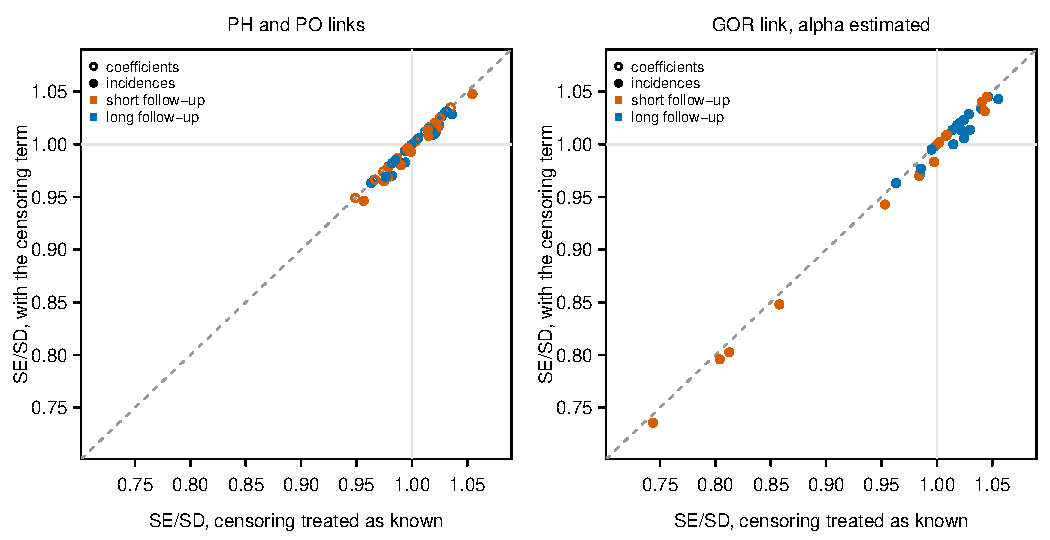
\includegraphics[width=0.85\textwidth]{figures/fig3_variance.pdf}
\caption{Study A. SE/SD with the variance of Proposition~\ref{prop:psi} (vertical axis) against the
variance treating the censoring distribution as known (horizontal), for every scenario and estimand.}
\label{fig:var}
\end{figure}

\subsection{Study B: three causes}\label{sec:simB}
\paragraph{Design.} With the same covariates, data were generated from two models. In the first
(\emph{constrained}), type 1 followed a Gompertz PH model ($\rho = -0.8$, $\tau = 0.5$,
$\beta = (0.5, -0.3)$), the remaining probability was shared between types 2 and 3 with
$\mathrm{logit}\,\pi_3 = -0.3 + 0.6 Z_1$, and $G_2$, $G_3$ were Weibull with shape 1.5 and scale
2, and shape 0.8 and scale 3. In the second (\emph{cause-specific}), the cause-specific hazards were
constant, $h_k(z) = \lambda_k \exp(g_k^\T z)$ with $\lambda = (0.12, 0.08, 0.05)$,
$g_1 = (0.5, -0.3)$, $g_2 = (0.3, 0)$, $g_3 = (-0.4, 0.3)$; then
$F_k(t \mid z) = h_k(z)/H(z)\,[1 - \exp\{-H(z)t\}]$ with $H = \sum_k h_k$, every subject has an
event, and a Cox model for each cause is correct while the constrained model is misspecified.
Censoring was uniform on $(0, c_{\max})$ with $c_{\max} = 12$ (long) or 5 (short); this censored 14\%
and 29\% under the first model and 27\% and 52\% under the second. $n = 500$ or 1500. We fitted the
constrained model ($K = 3$, Gompertz PH for type 1, Weibull $G_k$), the unconstrained joint model with
Gompertz PH models for all three types, and cause-specific Cox models.

\paragraph{Results.} Table~\ref{tab:B} and Figures~\ref{fig:coh} and \ref{fig:longrun}
summarise the long-run risks at $z = 0$. Under the constrained model, its estimator was
unbiased (largest absolute bias 0.005) with coverage 93.3--96.3\% for every type, scenario and
estimand, including the risks at $t_0 = 2$ (Table~\ref{tab:Bt0}). The unconstrained joint model, although
it contains the truth for type 1, was biased for all three types: with short follow-up the
long-run risk of type 2 was overestimated by 0.18--0.25 and that of type 3 underestimated by about
0.05, with coverage down to 37\%. More importantly, for 28--97\% of the subjects in a sample its
long-run risks added up to more than one, with sums up to 1.45; the constrained model never did
(Figure~\ref{fig:coh}). Under constant cause-specific hazards the constrained model was misspecified
and biased: for the long-run risks of type 3 with short follow-up the bias was 0.08--0.11 and
coverage fell to 28\% at $n = 1500$, and its risks at $t_0$ were biased by up to 0.02. The
cause-specific Cox models, correct in this scenario, were unbiased at $t_0$; they do not give long-run
risks without extrapolating the baseline hazards. Thus the constrained model is efficient and
coherent when its structure holds, but, as any parametric model, not robust to a different
structure; Section~\ref{sec:ident} and the application show how to check it.

\begin{table}[tbp]
\centering\scriptsize
\caption{Study B. Bias and coverage (\%) of the long-run risks $F_k(\infty \mid z = 0)$, and the
percentage of the subjects in a sample whose fitted long-run risks add up to more than one
(\% $>1$, averaged over replications) with the largest sum (Max). Coverage outside 93.6--96.4\% in
bold.}
\label{tab:B}
\setlength{\tabcolsep}{3.5pt}
\begin{tabular}{llll rr rr rr rr}
\toprule
 & & & & \multicolumn{2}{c}{Type 1} & \multicolumn{2}{c}{Type 2} & \multicolumn{2}{c}{Type 3} & \multicolumn{2}{c}{Coherence}\\
\cmidrule(lr){5-6}\cmidrule(lr){7-8}\cmidrule(lr){9-10}\cmidrule(lr){11-12}
Data & FU & $n$ & Model & Bias & Cov & Bias & Cov & Bias & Cov & \% $>1$ & Max \\
\midrule
Constrained & long & 500 & Constrained & $\phantom{-}0.000$ & 94.3 & $\phantom{-}0.001$ & 95.8 & $-0.001$ & 95.3 & 0 & 1.00 \\
 & &  & Joint & $\phantom{-}0.011$ & \textbf{90.8} & $\phantom{-}0.010$ & \textbf{92.0} & $-0.012$ & \textbf{89.8} & 52 & 1.22 \\
\addlinespace[2pt]
Constrained & long & 1500 & Constrained & $\phantom{-}0.000$ & 95.7 & $\phantom{-}0.000$ & 94.7 & $\phantom{-}0.000$ & \textbf{93.5} & 0 & 1.00 \\
 & &  & Joint & $\phantom{-}0.015$ & \textbf{86.3} & $-0.004$ & 93.7 & $-0.027$ & \textbf{65.2} & 28 & 1.13 \\
\addlinespace[2pt]
Constrained & short & 500 & Constrained & $\phantom{-}0.002$ & 94.7 & $\phantom{-}0.003$ & \textbf{93.3} & $-0.005$ & 93.6 & 0 & 1.00 \\
 & &  & Joint & $\phantom{-}0.006$ & 94.5 & $\phantom{-}0.252$ & \textbf{98.7} & $-0.042$ & \textbf{76.6} & 92 & 1.40 \\
\addlinespace[2pt]
Constrained & short & 1500 & Constrained & $\phantom{-}0.001$ & 94.8 & $\phantom{-}0.000$ & 93.8 & $-0.001$ & 95.1 & 0 & 1.00 \\
 & &  & Joint & $\phantom{-}0.006$ & 94.4 & $\phantom{-}0.184$ & \textbf{41.6} & $-0.052$ & \textbf{37.4} & 97 & 1.31 \\
\addlinespace[2pt]
Cause-specific & long & 500 & Constrained & $-0.020$ & \textbf{92.1} & $-0.002$ & 94.3 & $\phantom{-}0.022$ & \textbf{86.6} & 0 & 1.00 \\
 & &  & Joint & $\phantom{-}0.006$ & 96.1 & $-0.010$ & 94.7 & $\phantom{-}0.000$ & 95.0 & 70 & 1.25 \\
\addlinespace[2pt]
Cause-specific & long & 1500 & Constrained & $-0.018$ & \textbf{87.9} & $-0.004$ & 93.9 & $\phantom{-}0.022$ & \textbf{79.6} & 0 & 1.00 \\
 & &  & Joint & $-0.002$ & 94.3 & $-0.018$ & \textbf{86.9} & $-0.006$ & \textbf{93.4} & 58 & 1.19 \\
\addlinespace[2pt]
Cause-specific & short & 500 & Constrained & $-0.048$ & \textbf{87.3} & $-0.029$ & \textbf{76.0} & $\phantom{-}0.078$ & \textbf{57.4} & 0 & 1.00 \\
 & &  & Joint & $\phantom{-}0.062$ & \textbf{97.1} & $\phantom{-}0.020$ & \textbf{90.8} & $\phantom{-}0.077$ & \textbf{92.0} & 78 & 1.45 \\
\addlinespace[2pt]
Cause-specific & short & 1500 & Constrained & $-0.054$ & \textbf{71.0} & $-0.051$ & \textbf{63.3} & $\phantom{-}0.105$ & \textbf{27.6} & 0 & 1.00 \\
 & &  & Joint & $\phantom{-}0.030$ & \textbf{97.5} & $-0.013$ & \textbf{88.6} & $\phantom{-}0.018$ & \textbf{93.2} & 78 & 1.32 \\
\bottomrule

\end{tabular}
\end{table}

\begin{figure}[t]
\centering
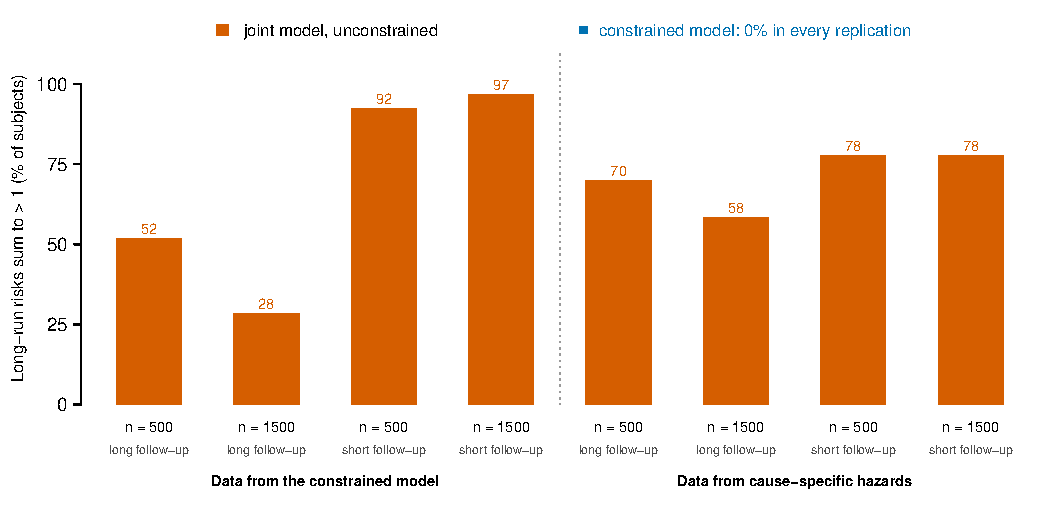
\includegraphics[width=\textwidth]{figures/fig1_coherence.pdf}
\caption{Study B. Percentage of subjects whose fitted long-run risks add up to more than one,
averaged over 1000 replications. The constrained model: 0\% in every replication by construction.}
\label{fig:coh}
\end{figure}

\begin{figure}[tbp]
\centering
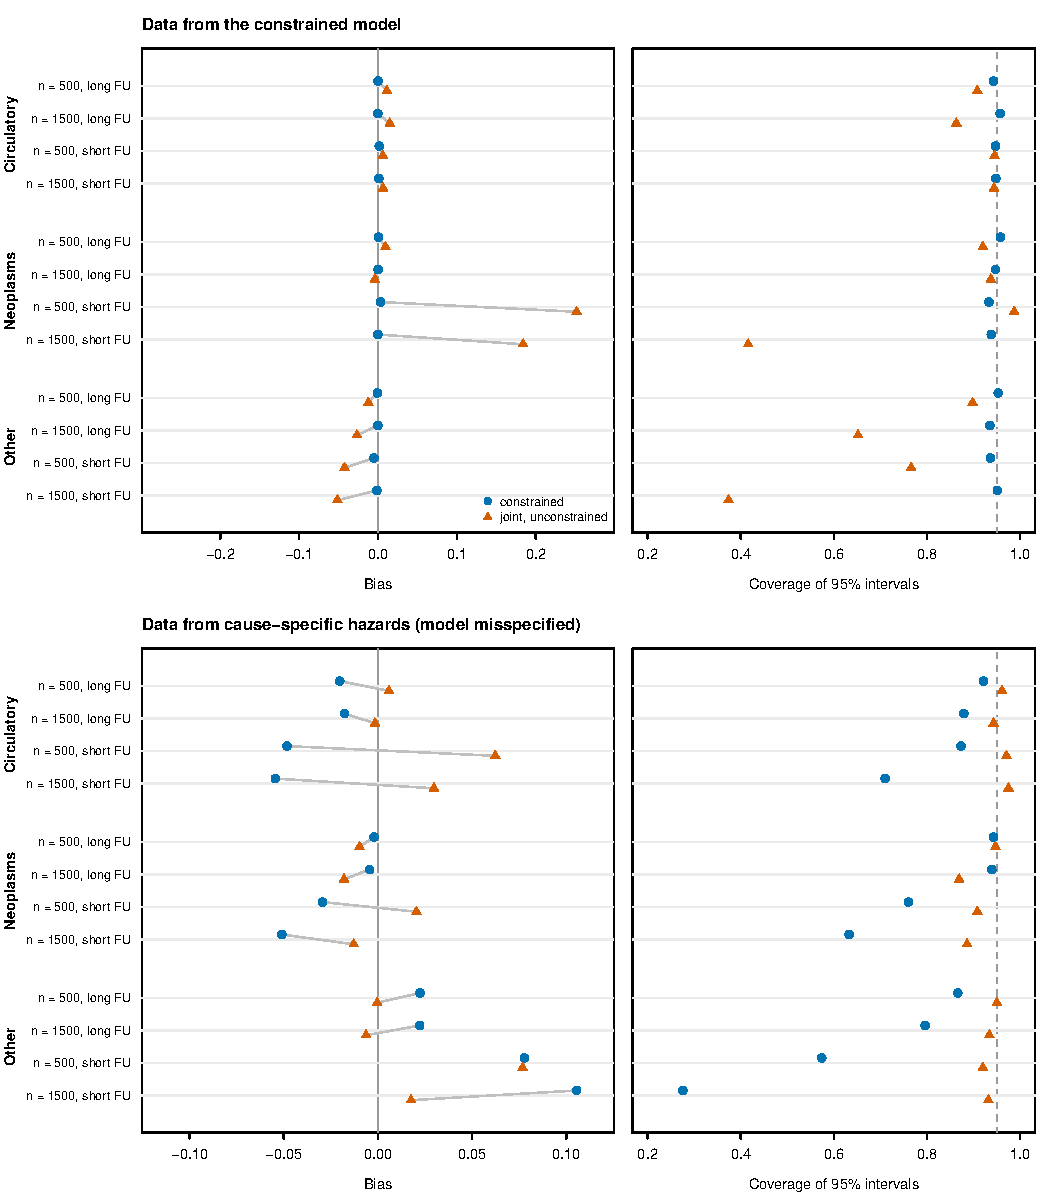
\includegraphics[width=0.92\textwidth]{figures/fig2_longrun.pdf}
\caption{Study B. Bias (left) and coverage of 95\% intervals (right) of the long-run risks at
$z = 0$, constrained against unconstrained joint model, under the constrained model (top) and under
constant cause-specific hazards (bottom). FU: follow-up.}
\label{fig:longrun}
\end{figure}

\subsection{Study C: computing time}\label{sec:time}
Table~\ref{tab:C} and Figure~\ref{fig:time} give seconds per fit on one data set of each size,
from Study A (two types) and Study B (three types), on \tbd{processor, R version}. With the PH
link the weighted estimator took 1.6 s for 50{,}000 subjects and grew roughly linearly, as
Section~\ref{sec:fast} predicts; with the PO link, without the suffix sums, it took 25 s. The
constrained three-type model took 0.7 s and the joint model 4.3 s. The semi-parametric Fine--Gray
estimator, which estimates a single coefficient vector without a baseline, was faster still.

\begin{table}[t]
\centering\small
\caption{Study C. Seconds per fit.}
\label{tab:C}
\begin{tabular}{r rrrrr}
\toprule
$n$ & Weighted PH & Weighted PO & Joint PH & Constrained ($K=3$) & Fine--Gray \\
\midrule
1{,}000 & 0.01 & 0.0192 & 0.0417 & 0.0132 & 0.0013 \\
5{,}000 & 0.0589 & 0.275 & 0.213 & 0.0663 & 0.00417 \\
20{,}000 & 0.34 & 4.07 & 1.12 & 0.275 & 0.0179 \\
50{,}000 & 1.57 & 24.9 & 4.33 & 0.67 & 0.05 \\
\bottomrule

\end{tabular}
\end{table}

\begin{figure}[t]
\centering
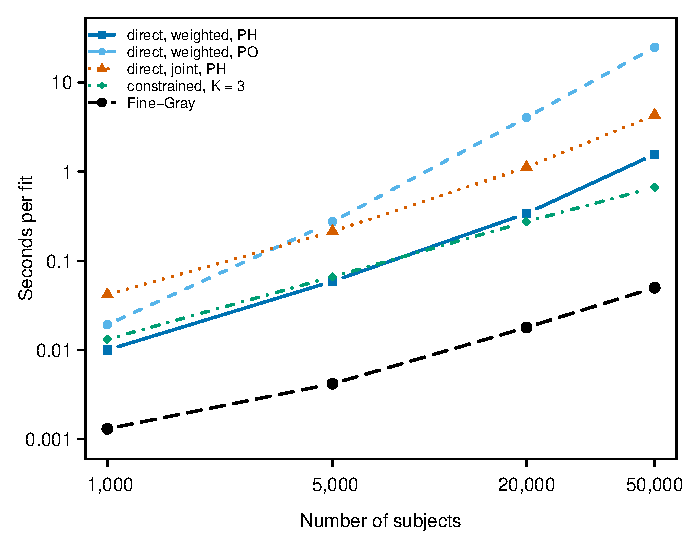
\includegraphics[width=0.55\textwidth]{figures/fig4_timing.pdf}
\caption{Study C. Seconds per fit against the number of subjects (log scales).}
\label{fig:time}
\end{figure}

\subsection{Validation of the implementation}\label{sec:valid}
The variance of Proposition~\ref{prop:psi} agreed with an independent implementation to $10^{-10}$
for every baseline and link, and with the numerical derivative of $\hat\theta(v)$ with respect to
the case weights, the Kaplan--Meier estimate recomputed, to the accuracy of the numerical
derivative ($1.5 \times 10^{-6}$). For the constrained model, $K = 2$ reproduced the two-cause model
of \citet{shi2013} to $10^{-13}$; the log-likelihood agreed with independent code to $10^{-12}$
and the score and information with numerical differentiation to $10^{-9}$ for $K = 3$ and 4.

% =====================================================================================
\section{Applications}\label{sec:apps}
% =====================================================================================
\subsection{Time to live birth}\label{sec:fert}
\citet{shayan2011} studied 652 married women aged 15--49 in rural Shiraz, Iran, recording the time
from marriage to the first live birth (type 1, 574 women), to a stillbirth or abortion (type 2, 33),
or to the end of follow-up (45 censored). We study the effect of education (illiterate 93,
primary or secondary 468, higher 91). Age was recorded at the end of follow-up and is therefore not
used as a covariate. Gray's test did not detect a difference between the education groups for either
type ($p = 0.13$ and 0.61).

For each type we fitted the weighted estimator with three baselines (Gompertz, Weibull mixture,
log-logistic mixture) and three links, and chose the fit with the largest $\ell_w$ minus the number of
parameters, a heuristic since $\ell_w$ is not a likelihood. For live birth this was the
log-logistic mixture with $\alpha$ estimated, $\hat\alpha = -0.34$ (95\% CI $-0.55$ to $-0.12$), so
that neither PH nor PO describes the data; the PH fit with the same baseline was close in $\ell_w$
minus parameters (difference 0.4). Women with higher education had a lower CIF of live birth at every
time than illiterate women ($e^{\hat\beta} = 0.62$, 95\% CI 0.45 to 0.85, on the generalized
odds-rate scale); the Fine--Gray estimate pointed the same way but was less precise (sHR 0.76, 0.56
to 1.03). The model gives the probability of ever having a live birth: 0.987 (SE 0.020), 0.937 (0.012)
and 0.857 (0.036) for the three education groups (Figure~\ref{fig:fert}), a summary the
semi-parametric model does not provide. For illiterate women, none of whom was censored, the
Aalen--Johansen estimate levels off at 0.95 and the model, which shares its baseline across groups,
is somewhat higher. For stillbirth or abortion the log-logistic mixture with the
PO link was chosen; education had no detectable effect (odds ratios 0.90 and 1.36 with wide
intervals), in agreement with the Fine--Gray model, and the long-run risk was about 5\%.

Censoring was light (7\%), and the variance correction changed the standard errors by at most
0.5\%. Because each type was fitted separately, nothing ties the two models together: for illiterate
women the two long-run risks add up to $0.987 + 0.055 = 1.04$, a mild form of the incoherence
that Section~\ref{sec:constrained} removes when all types are modelled together.

\begin{figure}[t]
\centering
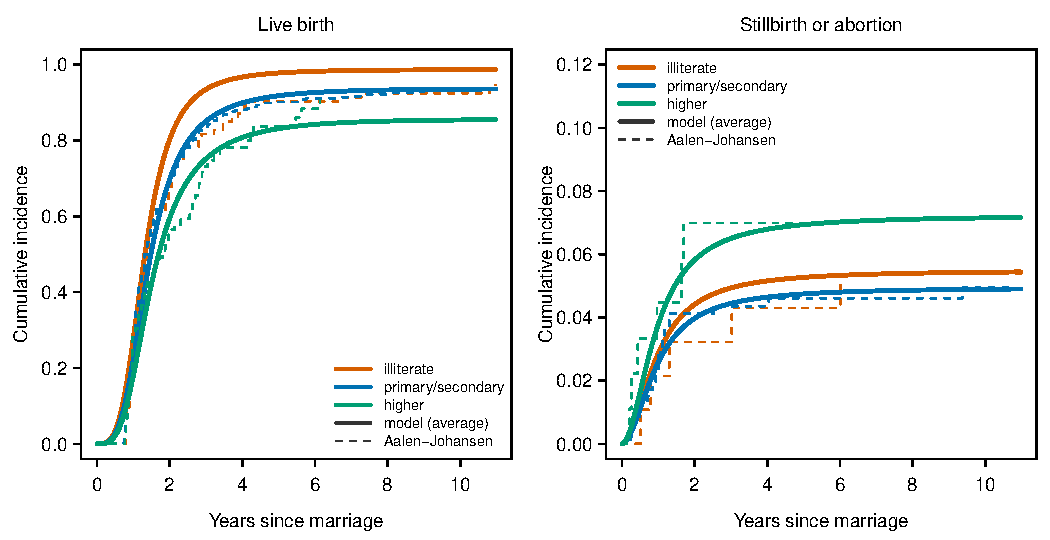
\includegraphics[width=\textwidth]{figures/fig7_fertility.pdf}
\caption{Time to live birth (left) and to stillbirth or abortion (right) by education: weighted
direct models (solid) and Aalen--Johansen estimates (dashed).}
\label{fig:fert}
\end{figure}

\subsection{Cause of death in the free light chain cohort}\label{sec:flchain}
The free light chain study followed residents of Olmsted County, Minnesota, aged 50 or more, for up
to 14 years after a serum sample \citep{kyle2006,dispenzieri2012}; the data are in the R package
\texttt{survival} \citep{survival}. We classified deaths as circulatory (type 1), neoplasms (type 2)
and other causes (type 3), and used age (per 5 years, centred), sex and a high total free light chain
(the two highest deciles) as covariates.

Long-run risks of death by cause are meaningful only if most subjects die within follow-up
(Section~\ref{sec:ident}). We therefore took as the main analysis the 765 subjects aged 80 or more at
enrolment, of whom 83\% died during follow-up (268 circulatory, 85 neoplasms, 285 other); the
subjects aged 70 or more and the whole cohort are sensitivity analyses. Among nine combinations of
baseline for type 1 and distribution $G_k$, AIC chose the modified logistic baseline with Weibull
$G_k$ (14 parameters); the Gompertz and Weibull-mixture baselines with Weibull $G_k$ were within
4--7 AIC units and gave nearly the same long-run risks (Table~\ref{tab:fl}). The parameter $c$ of the
modified logistic baseline was poorly determined (95\% CI $-5.8$ to 3.5), but the fitted CIFs and
long-run risks hardly depended on it.

\begin{table}[t]
\centering\small
\caption{Free light chain cohort, subjects aged 80 or more: constrained model (modified logistic PH
baseline for circulatory deaths, Weibull $G_k$). Type 1: subdistribution hazard ratios; type 3:
odds ratios of death from other causes rather than neoplasms among subjects who do not die of
circulatory disease.}
\label{tab:fl}
\begin{tabular}{lcc}
\toprule
 & Circulatory: sHR (95\% CI) & Other vs neoplasms: OR (95\% CI) \\
\midrule
Age (per 5 years) & 1.38 (1.20, 1.59) & 0.91 (0.64, 1.30) \\
Male              & 0.89 (0.68, 1.17) & 0.35 (0.21, 0.60) \\
High FLC          & 1.40 (1.09, 1.79) & 1.82 (1.06, 3.13) \\
\midrule
\multicolumn{3}{l}{Average long-run risk: circulatory 0.388, neoplasms 0.132, other 0.481 (sum 1)}\\
\multicolumn{3}{l}{Aalen--Johansen at 13.2 years: circulatory 0.372, neoplasms 0.118, other 0.404}\\
\multicolumn{3}{l}{Log-likelihood $-2467.6$, AIC 4963.2; other baselines: $\Delta$AIC 4.3 to 124}\\
\bottomrule
\end{tabular}
\end{table}

Older age and a high free light chain increased the CIF of circulatory death. Among those who did not
die of circulatory disease, men were less likely than women to die of other causes rather than of
neoplasms (OR 0.35), and a high free light chain made other causes more likely (OR 1.82). The fitted
long-run risks add up to one for every profile (Figure~\ref{fig:prof}); for an 85-year-old woman with a
normal free light chain they were 0.35, 0.13 and 0.52, and for a 90-year-old man with a high free
light chain 0.52, 0.14 and 0.34. The average fitted long-run risks exceeded the Aalen--Johansen
estimates at the end of follow-up by 0.016, 0.014 and 0.077 (Figure~\ref{fig:flcif}), as they should
when 17\% are still alive. At 10 years the constrained model agreed with cause-specific Cox models for circulatory deaths
(differences within 0.04 over the eight profiles). For the competing causes it agreed for
85-year-olds but gave lower 10-year risks for 90-year-olds: by 0.10--0.13 for other causes and up to
0.04 for neoplasms. Older subjects die sooner, and in \eqref{eq:ck} age can change how the remaining
probability is shared between the competing causes but not when those deaths occur, because the
$G_k$ do not depend on covariates. The long-run risks are not affected by this, the risks at fixed
times are. The unconstrained
joint model gave long-run risks adding up to more than one for every subject, with sums up to 2.27.

The sensitivity analyses show where long-run risks stop being identified. Among subjects aged 70 or
more (40\% alive at the end) the fitted long-run risk of neoplasms exceeded the Aalen--Johansen
estimate by 0.31, and in the whole cohort (73\% alive) by 0.68, while the other two types matched
closely: the probability of the survivors was assigned almost entirely to neoplasms, the type whose
Weibull $G$ had a decreasing hazard (shape 0.79--0.81) and hence the heaviest tail. Such long-run
risks are extrapolations of a parametric tail, and the check of Section~\ref{sec:ident} flags them.
CIFs within follow-up were unaffected (Figure~\ref{fig:flcif}, right).

\begin{figure}[t]
\centering
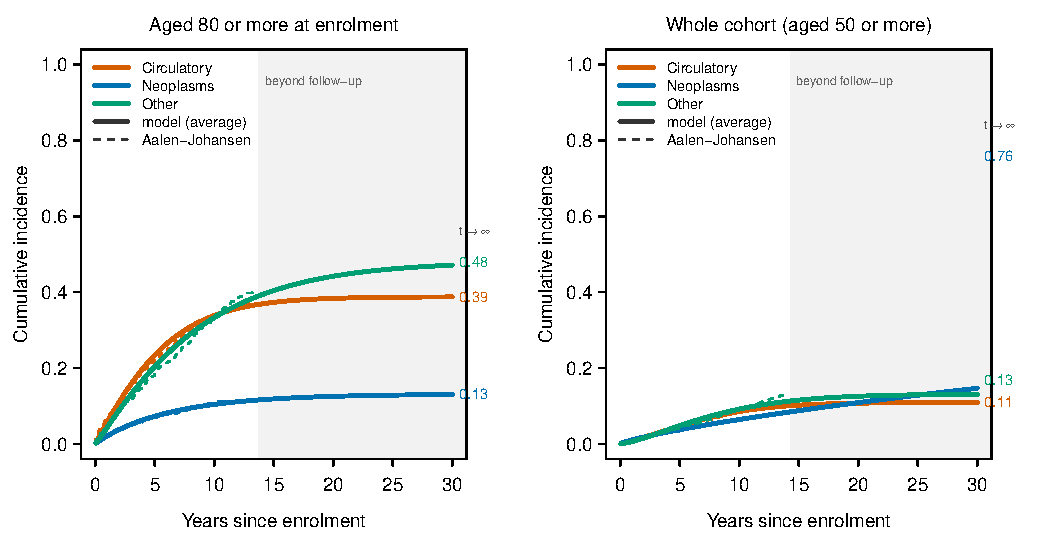
\includegraphics[width=\textwidth]{figures/fig5_flchain_cif.pdf}
\caption{Free light chain cohort. Average fitted CIFs of the constrained model (solid) and
Aalen--Johansen estimates (dashed), for subjects aged 80 or more (left) and the whole cohort (right);
values at the right margin are the long-run risks. Shaded: beyond follow-up.}
\label{fig:flcif}
\end{figure}

\begin{figure}[t]
\centering
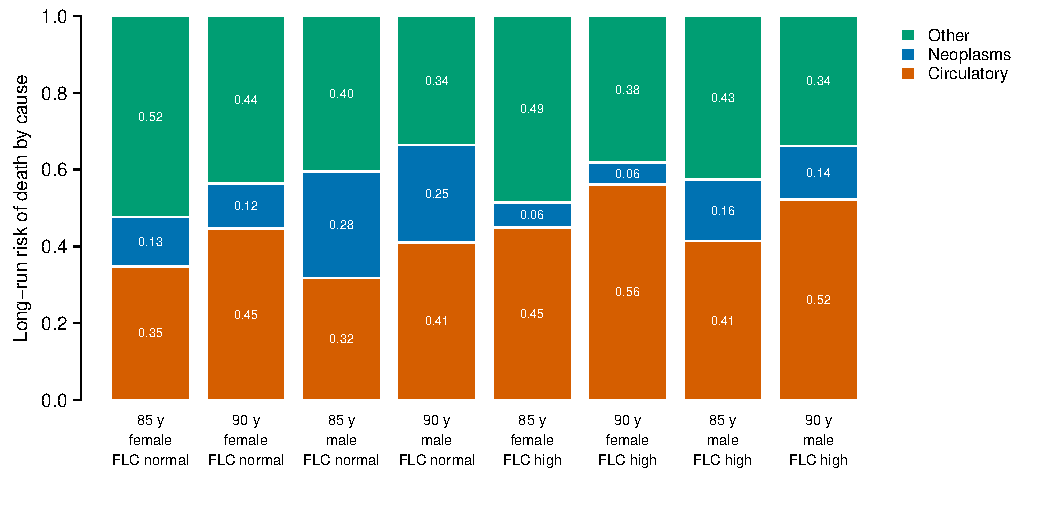
\includegraphics[width=\textwidth]{figures/fig6_flchain_profiles.pdf}
\caption{Free light chain cohort, aged 80 or more. Long-run risks of death by cause for eight
covariate profiles; by construction they add up to one.}
\label{fig:prof}
\end{figure}

% =====================================================================================
\section{Discussion}\label{sec:disc}
% =====================================================================================
We have studied two extensions of direct parametric regression for CIFs. The weighted estimator
needs no model for the competing causes, and in our simulations it was unbiased with nominal coverage
where the joint estimator, with one cause misspecified, was not; for the regression coefficients it
was as efficient as the Fine--Gray estimator while giving smooth CIFs and long-run risks. We derived
its variance with the estimated censoring distribution in closed form. The correction turned out to
be small, at most 1.2\% of the standard error, and it reduced rather than increased the standard
errors, as the projection argument predicts. We see this as a useful negative result: users of
weighted parametric estimators who ignore the estimation of the censoring distribution, as current
software does, obtain slightly conservative intervals. Larger effects may occur with heavier,
covariate-dependent or early censoring; covariate-dependent censoring would also require a
regression model for $G$, which we have not considered.

The constrained model makes the CIFs of all causes coherent by construction, for every covariate
value and at every time. When its structure holds it estimates long-run risks without bias, and the
unconstrained joint model, even when correctly specified for the cause of interest, does not.
Its structure is also its limitation. The competing causes share their time distributions across
covariate values, and the order of the causes matters: the cause of interest has a direct regression
model and the others are described by shares. Under constant cause-specific hazards it was biased,
and in the application it underestimated the 10-year risks of the competing causes for the oldest
subjects, whose deaths come sooner. The natural extension lets the $G_k$ depend on covariates, for
example through an accelerated failure time model; it keeps coherence, because
Proposition~\ref{prop:coherent} needs only that each $G_k(\cdot \mid z)$ is a distribution function,
at the price of more parameters when some type has few events. The model also assumes that everybody eventually has an event; when a
cured fraction is plausible the joint model with a constraint within follow-up, or a cure-model
formulation, is more appropriate.

Long-run risks are the main attraction of plateau baselines and their main risk. They are
identified only when follow-up is long enough for the CIFs to level off; otherwise they are
determined by the parametric tail. The comparison with the Aalen--Johansen estimate at the end of
follow-up is a simple guard, and the free light chain data show that it can fail badly for one cause
while the CIFs within follow-up remain good. Selection among baselines and links by the weighted
pseudo-likelihood is a heuristic; cross-validated prediction error \citep[Chapter~7]{hastie2009}
and information criteria for full likelihoods \citep{burnham2002} are available in \texttt{SurvX}
and give firmer ground. Finally, with the generalized odds-rate link the plateau and $\alpha$ are
hard to separate when follow-up is short; the long-run risks then had a heavy-tailed sampling
distribution.

\section*{Software and data availability}
{\sloppy
All methods are implemented in the R package \texttt{SurvX} \citep{ezzatabadipour2026}, function
\texttt{directcif()}: the weighted estimator with \texttt{estimation = "weighted"} (the variance of
Proposition~\ref{prop:psi} is the default) and the model of Section~\ref{sec:constrained} with
\texttt{estimation = "constrained"}. The fertility data are included in \texttt{SurvX} and the
free light chain data in \texttt{survival}. Code reproducing every table and figure is in the
supplementary material.\par}

\section*{Conflict of interest}
The author has declared no conflict of interest.

\bibliographystyle{apalike}
\bibliography{refs}

\appendix
% =====================================================================================
\section{Proof of Proposition~\ref{prop:psi}}\label{app:psi}
% =====================================================================================
Fix $\theta$ and a competing failure $j$ with first support index $f = f_j$. Its contribution to
$\ell_w$ is $L_j = \sum_{r = f}^{m+1} (\mu_r/\Ghat_{f-1}) \ell_{jr}$ with
$\ell_{jr} = \log S_1(c_r \mid Z_j)$. Since $\mu_r = \Ghat_{r-1} - \Ghat_r$ for $r \le m$ and
$\mu_{m+1} = \Ghat_m$, summation by parts gives
\[
L_j = \ell_{jf} + \sum_{r' = f}^{m} \frac{\Ghat_{r'}}{\Ghat_{f-1}}\,(\ell_{j,r'+1} - \ell_{jr'}),
\qquad \frac{\Ghat_{r'}}{\Ghat_{f-1}} = \exp\Big(\sum_{q=f}^{r'} \lambda_q\Big),
\]
so $L_j$ depends on the censoring distribution only through $\lambda_f, \dots, \lambda_m$, and
$\partial L_j / \partial\lambda_r = \I(f \le r) \sum_{r' \ge r} (\Ghat_{r'}/\Ghat_{f-1})(\ell_{j,r'+1} - \ell_{jr'})$.
Differentiating with respect to $\theta$ gives the contribution of $j$ to $Q_r = \partial U/\partial\lambda_r$
in \eqref{eq:Q}. The indices $f_j$ do not depend on $v$. Contributions of subjects with
$\delta_i \in \{0, 1\}$ do not depend on $\Ghat$.

With case weights, $\hat\theta(v)$ solves $\sum_i v_i U_i(\theta; \lambda(v)) = 0$. By the implicit
function theorem, at $v = 1$,
\[
\frac{\partial\hat\theta}{\partial v_i} = \hat A^{-1}\Big\{U_i + \sum_r \frac{\partial U}{\partial \lambda_r}\frac{\partial \lambda_r}{\partial v_i}\Big\}
= \hat A^{-1}(U_i + \psi_i).
\]
Finally $\lambda_r = \log(R_r - D_r) - \log R_r$, $\partial R_r/\partial v_i = Y_i(c_r)$ and
$\partial D_r/\partial v_i = \I(X_i = c_r, \delta_i = 0)$, which gives \eqref{eq:psi}. \qed

% =====================================================================================
\section{Score of the constrained model}\label{app:score}
% =====================================================================================
Write $q = 1 - p_1(z)$, $\Pi(t) = \sum_{k \ge 2} \pi_k(z) G_k(t)$, so that $S = 1 - F_1 - q\,\Pi$.
For an event of type $k \ge 2$ the log-density is $\log q + \log\pi_k + \log g_k$, with
$\partial \log q/\partial\theta_1 = -(\partial p_1/\partial\theta_1)/q$,
$\partial \log \pi_k / \partial(\gamma_j, \delta_j) = \{\I(j = k) - \pi_j\}(1, z^\T)$ and
$\partial \log g_k/\partial \phi_k$ that of the chosen distribution. For a censored subject,
\begin{gather*}
\frac{\partial \log S}{\partial \theta_1} = \frac{-\partial F_1/\partial\theta_1 + \Pi\,\partial p_1/\partial\theta_1}{S},\qquad
\frac{\partial \log S}{\partial \phi_k} = -\frac{q\,\pi_k\,\partial G_k/\partial\phi_k}{S},\\
\frac{\partial \log S}{\partial (\gamma_j, \delta_j)} = -\frac{q\,\pi_j\{G_j(t) - \Pi(t)\}}{S}(1, z^\T).
\end{gather*}
Second derivatives follow in the same way and are implemented analytically; both were checked
against numerical differentiation.

% =====================================================================================
\section{Supplementary tables}\label{app:tables}
% =====================================================================================
\begin{table}[h]
\centering\tiny
\caption{Study A, all estimands: SE/SD and coverage (\%), as ``SE/SD / coverage''. W and W$_0$:
weighted with and without the censoring term; WG and WG$_0$: the same with $\alpha$ estimated; J: joint;
FG: Fine--Gray.}
\label{tab:Afull}
\setlength{\tabcolsep}{2pt}
\begin{tabular}{llll cccccc}
\toprule
Link & FU & $n$ & Estimand & W & W$_0$ & WG & WG$_0$ & J & FG \\
\midrule
PH & long & 300 & $\beta_1$ & 1.01/95.5 & 1.01/95.5 & -- & -- & 0.69/\textbf{84.7} & 1.00/95.4 \\
PH & long & 300 & $\beta_2$ & 1.03/95.0 & 1.03/95.0 & -- & -- & 0.68/\textbf{82.9} & 1.03/94.9 \\
PH & long & 300 & $F_1(\infty\mid 0)$ & 1.01/94.9 & 1.02/95.2 & 1.01/95.1 & 1.02/95.3 & 0.61/\textbf{80.3} & -- \\
PH & long & 300 & $F_1(\infty\mid 1)$ & 0.98/94.5 & 0.99/94.9 & 1.00/95.3 & 1.01/95.5 & 0.67/\textbf{83.1} & -- \\
PH & long & 300 & $F_1(t_0\mid 0)$ & 1.03/95.3 & 1.03/95.3 & 1.05/96.3 & 1.05/96.4 & 0.73/\textbf{87.1} & -- \\
PH & long & 300 & $F_1(t_0\mid 1)$ & 1.00/94.5 & 1.00/94.5 & 1.02/94.9 & 1.02/95.1 & 0.83/\textbf{89.3} & -- \\
\addlinespace[2pt]
PH & long & 1000 & $\beta_1$ & 1.00/95.5 & 1.00/95.5 & -- & -- & 0.77/\textbf{89.0} & 1.00/95.3 \\
PH & long & 1000 & $\beta_2$ & 0.99/95.4 & 0.99/95.4 & -- & -- & 0.64/\textbf{74.2} & 0.99/95.1 \\
PH & long & 1000 & $F_1(\infty\mid 0)$ & 1.01/95.7 & 1.02/95.9 & 1.01/95.7 & 1.03/95.8 & 0.86/\textbf{90.0} & -- \\
PH & long & 1000 & $F_1(\infty\mid 1)$ & 0.97/94.4 & 0.98/94.5 & 0.97/94.4 & 0.98/94.6 & 0.81/\textbf{88.9} & -- \\
PH & long & 1000 & $F_1(t_0\mid 0)$ & 1.01/95.8 & 1.01/95.8 & 1.02/95.7 & 1.02/95.7 & 0.88/\textbf{90.6} & -- \\
PH & long & 1000 & $F_1(t_0\mid 1)$ & 0.96/94.1 & 0.96/94.1 & 0.96/94.2 & 0.96/94.4 & 0.86/\textbf{90.7} & -- \\
\addlinespace[2pt]
PH & short & 300 & $\beta_1$ & 1.02/95.4 & 1.02/95.4 & -- & -- & 0.98/94.6 & 1.02/95.5 \\
PH & short & 300 & $\beta_2$ & 0.97/94.7 & 0.97/94.7 & -- & -- & 0.87/\textbf{91.0} & 0.97/94.6 \\
PH & short & 300 & $F_1(\infty\mid 0)$ & 0.95/95.4 & 0.96/95.6 & 0.94/\textbf{96.5} & 0.95/\textbf{96.7} & 0.90/94.6 & -- \\
PH & short & 300 & $F_1(\infty\mid 1)$ & 0.98/95.7 & 0.99/96.0 & 1.03/96.3 & 1.04/\textbf{96.5} & 0.96/95.2 & -- \\
PH & short & 300 & $F_1(t_0\mid 0)$ & 0.98/94.8 & 0.98/94.8 & 1.00/95.3 & 1.00/95.3 & 0.94/94.1 & -- \\
PH & short & 300 & $F_1(t_0\mid 1)$ & 1.02/95.9 & 1.02/96.0 & 1.04/96.0 & 1.04/96.0 & 1.01/\textbf{96.5} & -- \\
\addlinespace[2pt]
PH & short & 1000 & $\beta_1$ & 1.00/94.8 & 1.00/94.8 & -- & -- & 0.97/94.1 & 0.99/94.7 \\
PH & short & 1000 & $\beta_2$ & 0.99/94.7 & 0.99/94.7 & -- & -- & 0.94/\textbf{89.6} & 0.99/94.8 \\
PH & short & 1000 & $F_1(\infty\mid 0)$ & 0.96/94.8 & 0.98/94.8 & 0.97/96.0 & 0.98/96.1 & 0.95/\textbf{91.5} & -- \\
PH & short & 1000 & $F_1(\infty\mid 1)$ & 0.97/95.1 & 0.98/95.4 & 0.98/96.1 & 1.00/96.2 & 0.96/93.7 & -- \\
PH & short & 1000 & $F_1(t_0\mid 0)$ & 1.00/94.8 & 1.00/94.8 & 1.00/95.2 & 1.00/95.2 & 0.98/94.2 & -- \\
PH & short & 1000 & $F_1(t_0\mid 1)$ & 1.00/94.3 & 1.00/94.4 & 1.00/94.7 & 1.00/94.7 & 0.99/94.3 & -- \\
\addlinespace[2pt]
PO & long & 300 & $\beta_1$ & 0.98/93.9 & 0.98/94.0 & -- & -- & 0.56/\textbf{73.9} & -- \\
PO & long & 300 & $\beta_2$ & 0.97/94.0 & 0.97/94.1 & -- & -- & 0.63/\textbf{78.3} & -- \\
PO & long & 300 & $F_1(\infty\mid 0)$ & 1.01/\textbf{96.6} & 1.02/\textbf{96.6} & 1.04/96.4 & 1.06/\textbf{96.6} & 0.54/\textbf{74.2} & -- \\
PO & long & 300 & $F_1(\infty\mid 1)$ & 0.97/94.0 & 0.98/94.2 & 0.98/94.5 & 0.99/94.7 & 0.67/\textbf{84.9} & -- \\
PO & long & 300 & $F_1(t_0\mid 0)$ & 1.01/95.2 & 1.01/95.2 & 1.02/95.7 & 1.02/95.7 & 0.59/\textbf{76.8} & -- \\
PO & long & 300 & $F_1(t_0\mid 1)$ & 0.99/94.2 & 0.99/94.2 & 0.99/94.5 & 1.00/94.5 & 0.77/\textbf{88.1} & -- \\
\addlinespace[2pt]
PO & long & 1000 & $\beta_1$ & 0.98/94.6 & 0.98/94.6 & -- & -- & 0.70/\textbf{83.9} & -- \\
PO & long & 1000 & $\beta_2$ & 1.01/94.7 & 1.01/94.7 & -- & -- & 0.71/\textbf{80.2} & -- \\
PO & long & 1000 & $F_1(\infty\mid 0)$ & 1.02/95.8 & 1.02/95.8 & 1.01/95.2 & 1.02/95.3 & 0.75/\textbf{84.5} & -- \\
PO & long & 1000 & $F_1(\infty\mid 1)$ & 1.03/95.0 & 1.04/95.3 & 1.03/95.4 & 1.04/95.4 & 0.94/\textbf{89.6} & -- \\
PO & long & 1000 & $F_1(t_0\mid 0)$ & 1.01/96.0 & 1.02/96.0 & 1.01/96.2 & 1.01/96.2 & 0.78/\textbf{85.6} & -- \\
PO & long & 1000 & $F_1(t_0\mid 1)$ & 1.03/95.9 & 1.03/95.9 & 1.03/95.5 & 1.03/95.5 & 0.88/\textbf{89.1} & -- \\
\addlinespace[2pt]
PO & short & 300 & $\beta_1$ & 1.02/95.7 & 1.03/95.7 & -- & -- & 0.97/94.5 & -- \\
PO & short & 300 & $\beta_2$ & 0.97/94.7 & 0.97/94.7 & -- & -- & 0.92/\textbf{92.4} & -- \\
PO & short & 300 & $F_1(\infty\mid 0)$ & 1.01/\textbf{97.3} & 1.01/\textbf{97.2} & 0.74/\textbf{97.9} & 0.74/\textbf{97.9} & 0.92/93.6 & -- \\
PO & short & 300 & $F_1(\infty\mid 1)$ & 0.99/95.5 & 1.00/95.6 & 0.80/\textbf{97.5} & 0.80/\textbf{97.5} & 0.98/94.8 & -- \\
PO & short & 300 & $F_1(t_0\mid 0)$ & 1.01/95.5 & 1.01/95.5 & 1.04/96.0 & 1.04/96.0 & 0.94/\textbf{93.3} & -- \\
PO & short & 300 & $F_1(t_0\mid 1)$ & 1.00/95.1 & 1.00/95.1 & 1.01/95.7 & 1.01/95.7 & 0.99/95.5 & -- \\
\addlinespace[2pt]
PO & short & 1000 & $\beta_1$ & 1.03/95.7 & 1.03/95.7 & -- & -- & 1.02/\textbf{93.1} & -- \\
PO & short & 1000 & $\beta_2$ & 0.95/\textbf{93.4} & 0.95/\textbf{93.4} & -- & -- & 0.91/\textbf{90.4} & -- \\
PO & short & 1000 & $F_1(\infty\mid 0)$ & 1.02/96.4 & 1.02/\textbf{96.5} & 0.80/\textbf{97.1} & 0.81/\textbf{97.2} & 0.96/\textbf{84.0} & -- \\
PO & short & 1000 & $F_1(\infty\mid 1)$ & 1.05/96.1 & 1.05/96.2 & 0.85/\textbf{97.0} & 0.86/\textbf{97.0} & 1.04/\textbf{93.4} & -- \\
PO & short & 1000 & $F_1(t_0\mid 0)$ & 1.00/94.2 & 1.00/94.3 & 1.01/94.5 & 1.01/94.5 & 0.96/\textbf{90.8} & -- \\
PO & short & 1000 & $F_1(t_0\mid 1)$ & 1.00/94.9 & 1.00/94.9 & 1.01/94.7 & 1.01/94.7 & 1.00/94.9 & -- \\
\bottomrule

\end{tabular}
\end{table}

\begin{table}[h]
\centering\scriptsize
\caption{Study B: CIFs at $t_0 = 2$ and $z = 0$. Bias, root mean squared error and coverage (\%).
Cause-specific Cox: point estimates only.}
\label{tab:Bt0}
\setlength{\tabcolsep}{3pt}
\begin{tabular}{llll rrr rrr rrr}
\toprule
 & & & & \multicolumn{3}{c}{Type 1} & \multicolumn{3}{c}{Type 2} & \multicolumn{3}{c}{Type 3}\\
\cmidrule(lr){5-7}\cmidrule(lr){8-10}\cmidrule(lr){11-13}
Data & FU & $n$ & Model & Bias & RMSE & Cov & Bias & RMSE & Cov & Bias & RMSE & Cov \\
\midrule
Constrained & long & 500 & Constrained & $-0.001$ & 0.030 & 94.5 & $\phantom{-}0.001$ & 0.023 & 94.4 & $\phantom{-}0.000$ & 0.018 & 95.1 \\
 & &  & Joint & $\phantom{-}0.008$ & 0.033 & \textbf{91.4} & $-0.008$ & 0.024 & 94.9 & $-0.007$ & 0.021 & \textbf{91.0} \\
 & &  & Cause-specific Cox & $\phantom{-}0.003$ & 0.031 & -- & $-0.002$ & 0.025 & -- & $-0.003$ & 0.020 & -- \\
\addlinespace[2pt]
Constrained & long & 1500 & Constrained & $\phantom{-}0.000$ & 0.017 & 94.5 & $\phantom{-}0.001$ & 0.013 & 95.8 & $\phantom{-}0.000$ & 0.010 & 95.0 \\
 & &  & Joint & $\phantom{-}0.015$ & 0.023 & \textbf{83.3} & $-0.008$ & 0.015 & \textbf{91.9} & $-0.008$ & 0.014 & \textbf{84.2} \\
 & &  & Cause-specific Cox & $\phantom{-}0.003$ & 0.018 & -- & $-0.002$ & 0.014 & -- & $-0.003$ & 0.011 & -- \\
\addlinespace[2pt]
Constrained & short & 500 & Constrained & $\phantom{-}0.000$ & 0.031 & 95.8 & $\phantom{-}0.000$ & 0.025 & 96.0 & $\phantom{-}0.000$ & 0.019 & 94.2 \\
 & &  & Joint & $\phantom{-}0.006$ & 0.032 & 94.8 & $-0.021$ & 0.031 & \textbf{89.4} & $-0.002$ & 0.021 & 95.1 \\
 & &  & Cause-specific Cox & $\phantom{-}0.003$ & 0.033 & -- & $-0.004$ & 0.027 & -- & $-0.003$ & 0.021 & -- \\
\addlinespace[2pt]
Constrained & short & 1500 & Constrained & $\phantom{-}0.000$ & 0.018 & 94.6 & $-0.001$ & 0.015 & 94.4 & $\phantom{-}0.000$ & 0.011 & 95.6 \\
 & &  & Joint & $\phantom{-}0.007$ & 0.019 & \textbf{92.5} & $-0.022$ & 0.026 & \textbf{66.6} & $-0.002$ & 0.012 & 94.6 \\
 & &  & Cause-specific Cox & $\phantom{-}0.002$ & 0.019 & -- & $-0.003$ & 0.016 & -- & $-0.002$ & 0.013 & -- \\
\addlinespace[2pt]
Cause-specific & long & 500 & Constrained & $\phantom{-}0.020$ & 0.029 & \textbf{82.7} & $\phantom{-}0.020$ & 0.027 & \textbf{77.0} & $\phantom{-}0.008$ & 0.017 & \textbf{91.0} \\
 & &  & Joint & $\phantom{-}0.011$ & 0.025 & \textbf{88.3} & $\phantom{-}0.008$ & 0.020 & \textbf{92.3} & $\phantom{-}0.002$ & 0.016 & 94.8 \\
 & &  & Cause-specific Cox & $-0.001$ & 0.023 & -- & $\phantom{-}0.001$ & 0.019 & -- & $\phantom{-}0.000$ & 0.016 & -- \\
\addlinespace[2pt]
Cause-specific & long & 1500 & Constrained & $\phantom{-}0.021$ & 0.024 & \textbf{56.4} & $\phantom{-}0.019$ & 0.022 & \textbf{52.5} & $\phantom{-}0.008$ & 0.012 & \textbf{85.0} \\
 & &  & Joint & $\phantom{-}0.017$ & 0.021 & \textbf{70.0} & $\phantom{-}0.008$ & 0.014 & \textbf{87.7} & $\phantom{-}0.002$ & 0.009 & 94.2 \\
 & &  & Cause-specific Cox & $-0.001$ & 0.013 & -- & $\phantom{-}0.000$ & 0.011 & -- & $\phantom{-}0.000$ & 0.010 & -- \\
\addlinespace[2pt]
Cause-specific & short & 500 & Constrained & $\phantom{-}0.013$ & 0.027 & \textbf{91.6} & $\phantom{-}0.016$ & 0.028 & \textbf{84.3} & $\phantom{-}0.007$ & 0.018 & \textbf{91.9} \\
 & &  & Joint & $\phantom{-}0.003$ & 0.024 & 95.4 & $\phantom{-}0.001$ & 0.022 & 94.3 & $-0.002$ & 0.018 & 94.8 \\
 & &  & Cause-specific Cox & $\phantom{-}0.001$ & 0.025 & -- & $\phantom{-}0.000$ & 0.023 & -- & $-0.002$ & 0.019 & -- \\
\addlinespace[2pt]
Cause-specific & short & 1500 & Constrained & $\phantom{-}0.011$ & 0.018 & \textbf{86.2} & $\phantom{-}0.014$ & 0.019 & \textbf{76.6} & $\phantom{-}0.007$ & 0.012 & \textbf{88.5} \\
 & &  & Joint & $\phantom{-}0.002$ & 0.014 & 94.4 & $\phantom{-}0.001$ & 0.012 & 95.0 & $\phantom{-}0.000$ & 0.010 & 95.8 \\
 & &  & Cause-specific Cox & $-0.001$ & 0.015 & -- & $\phantom{-}0.000$ & 0.013 & -- & $-0.001$ & 0.010 & -- \\
\bottomrule

\end{tabular}
\end{table}

\end{document}
